\documentclass[11pt,a4paper]{article} 
\usepackage{url}
\usepackage{mathpazo}
\usepackage{tikz}
\usetikzlibrary{calc}

% Layout
\textwidth=145mm
\textheight=230mm
\topmargin=0pt
\headheight=0pt
\oddsidemargin=10mm
\evensidemargin=0mm
\headsep=0pt
\parindent=0pt
\renewcommand{\baselinestretch}{1.1}
\setlength{\parskip}{0.3\baselineskip plus 1pt minus 1pt}

%%%%%%%%%%%%%%%%%%%%%%%%%%%%%%%%%%%%%%%%%%%%%%%%%%

\begin{document}

\title{\textbf The Slippery Slope of Conditional Probability}

\author{Moti Ben-Ari\\
Department of Science Teaching\\
Weizmann Institute of Science\\
\url{https://www.weizmann.ac.il/sci-tea/benari/}}

\maketitle

\begin{center}
\footnotesize\copyright{} Moti Ben-Ari $2023$
\end{center}
\vspace*{-3ex}
\begin{footnotesize}
This work is licensed under a Creative Commons Attribution-ShareAlike 4.0 International. To view a copy of this license, visit \url{http://creativecommons.org/licenses/by-sa/4.0/}.
\end{footnotesize}

%%%%%%%%%%%%%%%%%%%%%%%%%%%%%%%%%%%%%%%%%%%%%%%%%%

\section{Introduction}

When I told my colleague Prof. Abraham Arcavi that I had developed an interest in probability, he warned me that probability is a ``slippery'' subject, and I discovered that he was correct. And no concept in probability is as slippery as conditional probability, as exemplified by the famous Prisoners problem and the notorious Monty Hall problem \cite{carlton, fifty, jason, monty, three}. These problems are characterized by multiple interpretations of their presentations which lead to disputes (often acrimonious) concerning the correct solutions.

The article begins by presenting the Prisoners problem with an incorrect solution and then three correct solutions using conditional probability. These solutions are very similar but they show that different approaches lead to the same conclusion. Then it is shown how a bayesian interpretation of probability clarifies the Prisoners problem. The Monty Hall Problem is presented next with the rules given in complete detail in order to rule out non-canonical solutions. This is followed by a discussion of exactly how the Monty Hall problem is related to the Prisoners problem. I claim that the Monty Hall problem, too, should be studied from a bayesian interpretation. Finally, should the reader doubt the result, the results of a simulation are presented.

\textit{Terminology}: Mosteller uses the term \emph{Prisoner's dilemma}, which is widely used for a different problem in game theory. Carlton calls it the \emph{Prisoner's paradox}, but it is not really a paradox because the intuitive ``solution'' is based on an incorrect computation. Wikipedia's name \emph{Three prisoners problem} is preferable and I have shortened it to the \emph{Prisoners problem}.

\section{The Prisoners problem}

The first publication of the Prisoners problem was by Martin Gardner \cite{gardner}, but I prefer a slightly later version by Frederick Mosteller:
\begin{quote}
Three prisoners, $A,B$ and $C$, with apparently equally good records have applied for parole. The parole board has decided to release two of the three, and the prisoners know this but not which two. Prisoner $A$ realizes that it would be unethical to ask the warder if he, $A$, is to be released, but thinks of asking for the name of \emph{one} prisoner \emph{other than himself} who is to be released. He thinks that before he asks, his chances of release are $\frac{2}{3}$. He thinks that if the warder says ``$B$ will be released,'' his own chances have now gone down to $\frac{1}{2}$, because either $A$ and $B$ or $B$ and $C$ are to be released. And so $A$ decides not to reduce his chances by asking. However, $A$ is mistaken in his calculations. Explain \cite[Problem~13, emphasis in the original]{fifty}.
\end{quote}
In the sequel we use the name of a prisoner $\{A,B,C\}$ for the event that that prisoner will be released.

%%%%%%%%%%%%%%%%%%%%%%%%%%%%%%%%%%%%%%%%%%%%%%%%%%

\section{Solution 1}

The presentation of the problem does not specify the criteria that will be used to decide whom to release. However, the expression ``apparently equally good records'' should be interpreted so that there is an equal probability of $\frac{2}{3}$ that each prisoner will be released, as noted later in the problem.

The probability that $A$ will be released conditional upon the probability that $B$ will be released is:
\[
P(A|B) = \frac{P(A\cap B)}{P(B)} = \frac{1/3}{2/3}=\frac{1}{2}\,.
\]
However, the new information is \emph{not} that $B$ will be released but that the warder \emph{tells} $A$ that $B$ will be released. Therefore, we cannot accept this solution.

\section{Solution 2}

A correct solution can be obtained by carefully identifying the possible events, which can be displayed in a diagram (Figure~\ref{f.prisoners}).
\begin{figure}
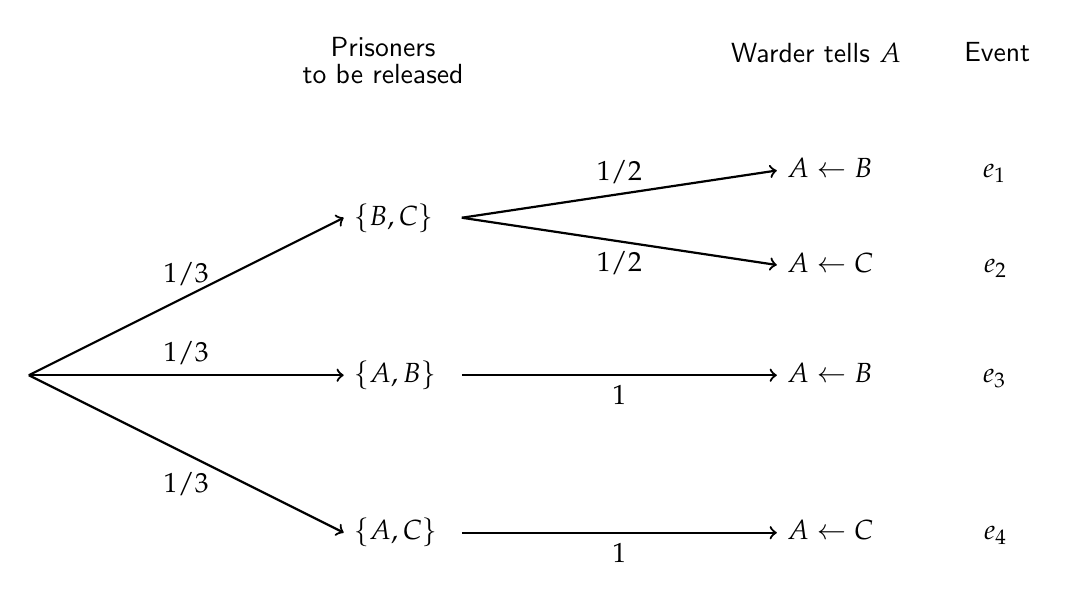
\begin{tikzpicture}
\coordinate (root) at (0,0);
\draw[thick,->] (root) -- node[above] {$1/3$} (4,2)
  coordinate(top) node[right] {$\{B,C\}$};
\draw[thick,->] (root)-- node[above] {$1/3$} (4,0)
   coordinate(middle) node[right] {$\{A,B\}$};
\draw[thick,->] (root)-- node[below,yshift=-3pt] {$1/3$} (4,-2)
  coordinate(bottom) node[right]  {$\{A,C\}$};
\draw[thick,->] ($(top)+(1.5,0)$) --
  node[above] {$1/2$} +(4,.6)
  coordinate(one) node[right] {$A\leftarrow B\qquad\qquad e_1$};
\draw[thick,->] ($(top)+(1.5,0)$) --
  node[below] {$1/2$} +(4,-.6)
  coordinate(two) node[right] {$A\leftarrow C\qquad\qquad e_2$};
\draw[thick,->] ($(middle)+(1.5,0)$) --
  node[below] {$1$}  +(4,0) 
  coordinate(three) node[right] {$A\leftarrow B\qquad\qquad e_3$};
\draw[thick,->] ($(bottom)+(1.5,0)$) --
  node[below] {$1$} +(4,0)
  coordinate(four) node[right] {$A\leftarrow C\qquad\qquad e_4$};
\node at ($(top)+(.5,2)$) {\textsf{\shortstack{Prisoners\\to be released}}};
\node at ($(one)+(.5,1.5)$) {\textsf{Warder tells $A$}};
%\node at ($(one)+(-.5,1.5)$) {\textsf{\shortstack{Warder tells $A$\\who will be released}}};
\node at ($(one)+(2.8,1.5)$) {\textsf{Event}};
\end{tikzpicture}
\caption{Probability tree for the Prisoners problem}\label{f.prisoners}
\end{figure}
There are four mutually exclusive events:
\begin{description}
\item[$e_1$:] $\{B,C\}$ are to be released and $A$ is told that $B$ will be released.
\item[$e_2$:] $\{B,C\}$ are to be released and $A$ is told that $C$ will be released.
\item[$e_3$:] $\{A,B\}$ are to be released and $A$ is told that $B$ will be released.
\item[$e_4$:] $\{A,C\}$ are to be released and $A$ is told that $C$ will be released.
\end{description}
The event that $B$ and $C$ will be released is $e_1\cup e_2$.

Assuming that the release of each prisoner is determined independently of the others, the probability of each pair will be released is:
\[
P(e_1)=P(e_2)=P(e_3\cup e_4)=\frac{1}{3}\,.
\]

We now make an additional assumption that does not appear in the problem: if $\{B,C\}$ are to be released, $A$ is told correctly whether $B$ or $C$ will be released and with equal probability, so:
\[
P(e_1)=P(e_2)=\frac{1}{2}\cdot \frac{1}{3}=\frac{1}{6}\,.
\]
The probability that $A$ will be released conditional upon $A$ being told that $B$ will be released is:
\[
P(e_3\cup e_4|e_1\cup e_3) = \frac{P((e_3\cup e_4)\cap(e_1\cup e_3))}{P(e_1\cup e_3)}=\frac{P(e_3)}{P(e_1\cup e_3)}=\frac{1/3}{(1/3)+(1/6)}=\frac{2}{3}\,.
\]
That $P((e_3\cup e_4)\cap(e_1\cup e_3))=P(e_3)$ can be shown using Venn diagrams or the distributed law for sets.

The additional information that $A$ obtains from the warder does not change the probability that he will be released.

%%%%%%%%%%%%%%%%%%%%%%%%%%%%%%%%%%%%%%%%%%%%%%%%%%

\section{Solution 3}

We approach this solution using conditional probability but with the correct additional information. Denote the event that $A$ is \emph{told} by the warder that $B$ will be released by $A\leftarrow B$. The formula for the conditional probability is now:
\[
P(A|(A\leftarrow B))=\frac{P(A\cap (A\leftarrow B))}{P(A\leftarrow B)}
\]
In order to compute $P(A\cap (A\leftarrow B))$ we need to ask: under what conditions will $A$  be released \emph{and} the warder tells him that $B$ will be released. $A$ asks the warder for the name of one of the prisoners who will be released, so we can assume that the warder knows who they are. Of course, he could lie so we also have to assume that he tells the truth. Therefore:
\[
P(A\cap (A\leftarrow B))=P(\{A,B\})=\frac{1}{3}\,.
\]
Next, we assume that if $\{B,C\}$ are to be released, the warder will tell $A$ that $B$ or $C$ will be released with equal probability so:
\[
P(A\leftarrow B)=P(\{A,B\})+\frac{1}{2} P(\{B,C\})=\frac{1}{3}+\frac{1}{2}\cdot\frac{1}{3}=\frac{1}{2}\,.
\]
The probability that $A$ will be released if he is told that $B$ will be released is:
\[
P(A|(A\leftarrow B)) =\frac{P(A\cap (A\leftarrow B))}{P(A\leftarrow B)} = \frac{1/3}{1/2}=\frac{2}{3}\,.
\]

%%%%%%%%%%%%%%%%%%%%%%%%%%%%%%%%%%%%%%%%%%%%%%%%%%

\section{Solution 4}

The probability can be solved using Bayes' theorem:
\[
P(A|A\leftarrow B)= \frac{P(A\leftarrow B|A)\,P(A)}{P(A\leftarrow B)}\,,
\]
where:
\begin{itemize}
\item The priori probability $P(A)$ was specified to be $2/3$.
\item $P(A\leftarrow B|A)=1/2$ since if $A$ is released then either $B$ or $C$ will also be released with equal probability.
\item $P(A\leftarrow B)=1/2$ as shown in Solution~3.
\end{itemize}
The posteriori probability is:
\[
P(A|A\leftarrow B)= \frac{P(A\leftarrow B|A)\,P(A)}{P(A\leftarrow B)} = \frac{(1/2)(2/3)}{1/2}=\frac{2}{3}\,.
\]

\section*{Summary of the Prisoners problem}

The three solutions approach the problem in different ways but result in similar (simple) formulas for the conditional probability. A careful application of conditional probability is all that is needed to solve the problem.

There are four assumptions that are not \emph{explicitly} written in the problem but are crucial if one wants to obtain the canonical solution:
\begin{itemize}
\item The choice by the parole board of which pair of prisoners to release is random with equal probability.
\item The warder knows the identity of the prisoners who will be released.
\item If $\{B,C\}$ are to be released he tells $A$ that $B$ or $C$ will be released with equal probability.
\item The warder tells $A$ the truth.
\end{itemize}

%%%%%%%%%%%%%%%%%%%%%%%%%%%%%%%%%%%%%%%%%%%%%%%%%%

\section{The bayesian interpretation of probability}

$A$'s dilemma concerning the probability that he will be released makes no sense. When the warden tells $A$ the name of another prisoner to be released, the decision has \emph{already} been made, so what does ``probability'' mean?

The intuitive (non-axiomatic) definition of probability is that $P(E)$, the probability that an event $E$ occurs, is the proportion of time that $E$ occurs in a large number of trials.  This interpretation is the \emph{frequentist interpretation} of probability which is essentially a prediction that, for example, if you throw a fair die $6000$ times, $6$ will appear $1000$ times, more or less, as formalized by the Law of Large Numbers.  

But the Prisoners problem concerns a single trial: the release of two out of three specific prisoners on a specific day. The frequentist interpretation is therefore unable to make sense of the Prisoners problem as posed, though it would make sense as an abstract problem asking for a prediction of the result of a long series of trials.

Probabilistic reasoning was used to investigate the author of each of the Federalist Papers, but what does this mean in the frequentist interpretation?
\begin{quote}
The problem, as [Mosteller] saw it, was that treating a \emph{unique event} like ``Hamilton wrote paper No. 52'' was difficult with sampling theory \cite[p.~156, my emphasis]{mcgrayne}.
\end{quote}

The Prisoners problem should be interpreted according the \emph{bayesian interpretation} of probability, which in this case is asking how $A$'s \emph{belief} in his future release is changed by the additional information that $B$ will be released. The solutions show that he has no justification for changing his belief. The bayesian interpretation is implicit in the usual formulations of the Prisoners problem:
\begin{quote}
[$A$] \emph{thinks} that if the warder says ``B will be released,'' \emph{his own chances} have now gone down to $\frac{1}{2}$, because either $A$ and $B$ or $B$ and $C$ are to be released \cite[p.~4, my emphasis]{fifty}.
\end{quote}
The use of ``thinks'' and ``his own chances'' is a clear indication that the bayesian interpretation is intended, because in the frequentist interpretation probability is objective, not what you think it is and no one owns a probability.

%%%%%%%%%%%%%%%%%%%%%%%%%%%%%%%%%%%%%%%%%%%%%%%%%%

\section{The Monty Hall problem}

The Monty Hall problem is extremely famous; I won't write about its history, which is readily available, for example, on Wikipedia \cite{monty}. Rivers of ink have been spilled discussing interpretations of the problem caused by misunderstandings, as well as by interpretations that lead to different problems \cite{jason}.

\subsection*{Posing the problem}
The problem is posed in the context of a game show and its first publication was by Selvin \cite{selvin}:\footnote{Selvin expresses the problem as a dialogue between the host and the contestant. Here I give a version in prose that is consistent with Selvin's presentation, but similar to how the problem is currently posed.}
\begin{quote}
There are three doors $A, B, C$. There is a car behind one door and goats behind the other two. If you choose the door with the car you win the card. Choose one of the doors. (You choose door $B$.) Remember that the probability that door $B$ contains the car is $1/3$ and the probability that it contains a goat is $2/3$.

I'll do  you a favor and open one of the remaining doors. (Opens door $A$.) There is a goat there! Since there are two doors left, the probability of that there is a car behind the door you chose is $1/2$. (You change your choice and ask that door $C$ be opened.)
\end{quote}
Is the host correct that the probability is $1/2$, in which case it doesn't matter if you change your choice or not, or are you correct in wanting to change your choice?

The canonical solution depends of clarifying what the host and the contestant must do and what is probabilistic, so I give the rules of the game and the (implicit) assumptions in excruciating detail:
\begin{enumerate}
\item In a game show there are three doors and three prizes, a car and two goats.
\item The prizes are randomly placed behind each door with equal probability.
\item The contestant prefers to win the car and not a goat!
\item The host knows which prize is behind each door.
\item The contestant must choose one door. The choice is random with equal probability.
\item The host must open one of the doors with a goat. There are two possibilities:
\begin{itemize}
\item If the contestant chose the door with the car, the host must open one of the two doors with goats and the choice is random with equal probability.
\item If the contestant chose a door with a goat, the host must open the door with the second goat. 
\end{itemize}
\item After the door is opened, the contestant must decide whether to stay with the door he originally chose or to choose the other unopened door.
\item The host opens the door that was chosen (either the original choice or after he changes his choice) and the contestant wins the prize behind that door.
\end{enumerate}
What is the probability that the contestant wins the car if he stays with his original choice? What is the probability that the contestant wins the car if he changes his choice?

\subsection*{Comparison with the Prisoners problem}

Consider a variation on the Monty Hall game where the contestant is \emph{not} allowed to change his choice! Just as in the Prisoners problem, where the information that the warder tells the prisoner cannot affect the probability, here, too, opening the door changes nothing. The probability $1/3$ that the contestant wins with his original choice is unchanged. In the original Monty Hall problem it is only because the contestant is allowed to change his choice that opening the door has any meaning.

\subsection*{Bayesian interpretation}

As with the Prisoners problem, the Monty Hall problem as posed makes no sense in a frequentist interpretation of probability because the problem asks about a single trial. The usual presentations of the problem do not ask for probabilities, rather, they ask for a strategy. Is it to the contestant's advantage to change his choice? This implies that a bayesian interpretation of probability as belief is intended. Does the additional information obtained by the opening of a door increase or decrease the contestant's belief in the position of the car or does it not affect it at all?

%%%%%%%%%%%%%%%%%%%%%%%%%%%%%%%%%%%%%%%%%%%%%%%%%%

\section{Solution of the Monty Hall problem}

As with the Prisoners problem the Monty Hall problem can be solved in several different, but similar, ways. Here we bring a solution obtained by identifying events as in Solution~2 to the Prisoners problem. The reader is invited to solve the problem using the other two approaches.

Figure~\ref{f.monty-hall} shows the events and the probabilities which have been constructed according to the rules. The car is randomly placed behind one of the doors (rule~1) and the contestant randomly chooses a door (rule~5). The host knows where the goats are (rule~4) and he must open a door with a goat (rule~6). If the car is behind door~1, he must choose randomly to open door two or three (rule~6a); otherwise, he must choose the remaining door (rule~6b).

The possible events are (Figure~\ref{f.monty-hall}):\footnote{Note the similarity of this figure to Figure~\ref{f.prisoners}.}

\begin{figure}
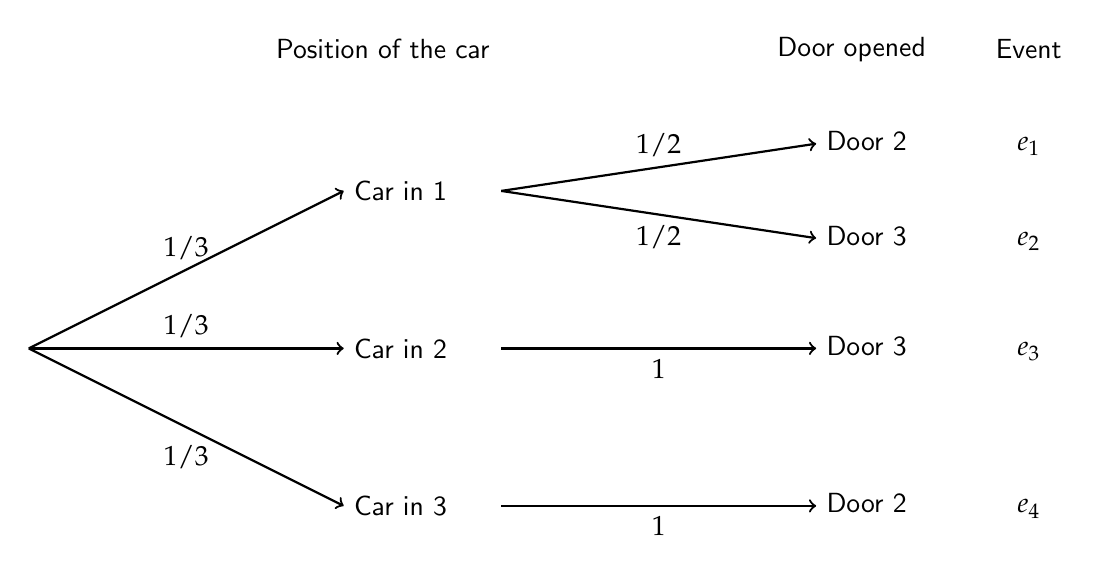
\begin{tikzpicture}
\coordinate (root) at (0,0);
\draw[thick,->] (root) -- node[above] {$1/3$} (4,2)
  coordinate(top) node[right] {\textsf{Car in 1}};
\draw[thick,->] (root)-- node[above] {$1/3$} (4,0)
   coordinate(middle) node[right] {\textsf{Car in 2}};
\draw[thick,->] (root)-- node[below,yshift=-3pt] {$1/3$} (4,-2)
  coordinate(bottom) node[right]  {\textsf{Car in 3}};
\draw[thick,->] ($(top)+(2,0)$) --
  node[above] {$1/2$} +(4,.6)
  coordinate(one) node[right] {\textsf{Door 2}$\qquad\qquad e_1$};
\draw[thick,->] ($(top)+(2,0)$) --
  node[below] {$1/2$} +(4,-.6)
  coordinate(two) node[right] {\textsf{Door 3}$\qquad\qquad e_2$};
\draw[thick,->] ($(middle)+(2,0)$) --
  node[below] {$1$}  +(4,0) 
  coordinate(three) node[right] {\textsf{Door 3}$\qquad\qquad e_3$};
\draw[thick,->] ($(bottom)+(2,0)$) --
  node[below] {$1$} +(4,0)
  coordinate(four) node[right] {\textsf{Door 2}$\qquad\qquad e_4$};
\node at ($(top)+(.5,1.8)$) {\textsf{Position of the car}};
\node at ($(one)+(.45,1.2)$) {\textsf{Door opened}};
\node at ($(one)+(2.7,1.2)$) {\textsf{Event}};
\end{tikzpicture}
\caption{Probability tree for the Monty Hall problem}\label{f.monty-hall}
\end{figure}
\begin{itemize}
\item $e_1$: the car is behind door 1 and the host opens door 2.
\item $e_2$: the car is behind door 1 and the host opens door 3.
\item $e_3$: the car is behind door 2 and the host opens door 3.
\item $e_4$: the car is behind door 3 and the host opens door 2.
\end{itemize}
Without loss of generality assume that the contestant chooses door~1. In events $e_1, e_2$, the probability that the contestant wins the car if he does not change his choice is:
\[
P_{\textsf{\scriptsize no change}}(\textsf{win})=P(e_1)+P(e_2)=\frac{1}{3}\cdot\frac{1}{2}+\frac{1}{3}\cdot\frac{1}{2}=\frac{1}{3}\,.
\]
In events $e_3,e_4$, the probability that the contestant wins the car if he changes his choice is:
\[
P_{\textsf{\scriptsize change}}(\textsf{win})=P(e_3)+P(e_4)=\frac{1}{3}\cdot 1+\frac{1}{3}\cdot 1=\frac{2}{3}\,.
\]
Therefore, the optimal strategy for the contestant is to change his choice of door, raising the probability of winning the car from $1/3$ to $2/3$.

Again, the frequentist probabilities don't change: the probability is $1/3$ that the car is behind the door the contestant originally chose and the probability is $2/3$ that it is behind the other two doors. However, this $2/3$ is now ``concentrated'' in the one door that remains closed and, therefore, according to the bayesian interpretation, the contestant's belief that the car is behind the other door has doubled and his strategy should be to change his choice.

%%%%%%%%%%%%%%%%%%%%%%%%%%%%%%%%%%%%%%%%%%%%%%%%%%

\section{Simulation of the Monty Hall problem}

Andrew Vazsonyi reports that when he showed the problem to Paul Erd\H{o}s, he initially refused to accept the answer \cite[p.~17]{erdos}. Only after Vazsonyi showed him a simulation, did Erd\H{o}s accept that the answer was correct. If a luminary like Paul Erd\H{o}s found the solution hard to accept, we shouldn't expect that students will find it easier to understand.

Monte Carlo simulations are an excellent way to become convinced of the correctness of a computation in probability. The following short program in the Python programming language simulates the problem:
\renewcommand{\baselinestretch}{1.1}
\begin{verbatim}
import random
n      = 10000  # Number of simulations
stay   = 0      # Games won by staying
change = 0      # Games won by changing
for i in range(n):
    doors = [False, False, False]
    doors[random.randint(0,2)] = True
    if     doors[0]: stay   += 1
    if not doors[0]: change += 1
print('Stay   = {:.4f}'.format(stay   / n))
print('Change = {:.4f}'.format(change / n))
\end{verbatim}
The result of the simulation is that the proportions of wins when staying is $0.335$ and the proportion of wins when changing is $0.665$. A simulation makes sense in the frequentist interpretation of probability. If the contestant were familiar with the problem and the result of a simulation, he could decide whether to change or not based on these results. 

%%%%%%%%%%%%%%%%%%%%%%%%%%%%%%%%%%%%%%%%%%%%%%%%%%

\section{Conclusion}

Conditional probability is a concept that students find difficult to understand. The Prisoners problem and the Monty Hall problem can facilitate understanding, since the computations in involved are simple and yet there are non-trivial difficulties in formulating solutions. 

This article shows that the problems can be easily solved by approaches that  require a careful application of conditional probability. It identifies a link between the Prisoners problem and the Monty Hall problem. Most importantly, it claims that the bayesian interpretation facilitates understanding these problems.

%%%%%%%%%%%%%%%%%%%%%%%%%%%%%%%%%%%%%%%%%%%%%%%%%%

\subsection*{Acknowledgments}
I would like to thank Avital Elbaum-Cohen, David Fortus, Aaron M. Montgomery and Gila Ron for their comments on this article.

%%%%%%%%%%%%%%%%%%%%%%%%%%%%%%%%%%%%%%%%%%%%%%%%%%

\begin{thebibliography}{10}

%\bibitem{bt}
%Dimitri P. Bertsekas , John N. Tsitsiklis.
%\newblock \textit{Introduction To Probability (2nd Edition)}.
%\newblock Athena Scientific, 2008.

\bibitem{BW}
Joseph K. Blizstein and Jessica Hwang.
\newblock  \textit{Introduction to Probability (Second Edition)}.
\newblock CRC Press, 2019.

\bibitem{carlton}
Matthew Carlton.
\newblock Pedigrees, prizes, and prisoners: The misuse of conditional
  probability.
\newblock \textit{Journal of Statistics Education}, 13(2), 2005.
\newblock \url{https://doi.org/10.1080/10691898.2005.11910554}.

\bibitem{gardner}
Martin Gardner. 
\newblock Mathematical games: Problems involving questions of probability and ambiguity. 
\newblock \textit{Scientific American}
\newblock 201(4), 174–182, 1959.

\bibitem{mcgrayne}
Sharon Bertsch McGrayne.
\newblock \textit{The Theory That Would Not Die : How Bayes' Rule Cracked the Enigma Code, Hunted down Russian Submarines, and Emerged Triumphant from Two Centuries of Controversy}.
\newblock Yale University Press, 2011.

\bibitem{fifty}
Frederick Mosteller.
\newblock \textit{Fifty Challenging Problems in Probability with Solutions}.
\newblock Dover, 1965.

\bibitem{jason}
Jason Rosenhouse.
\newblock  \textit{The Monty Hall Problem: The Remarkable Story of Math's Most Contentious Brainteaser}.
\newblock Oxford University Press, 2009.

\bibitem{selvin}
Steven Selvin. 
\newblock A problem in probability.
\newblock \textit{The American Statistician}.
\newblock 29(1), 67–71, 1975.

\bibitem{erdos}
Andrew Vazsonyi.
\newblock Which Door Has the Cadillac?
\newblock \textit{Decision Line},
\newblock 1998-1999, 17–19.
\newblock \par\noindent\url{https://web.archive.org/web/20140413131827/http://www.decisionsciences.org/DecisionLine/Vol30/30_1/vazs30_1.pdf}.

\bibitem{monty}
Wikipedia.
\newblock \textit{Monty Hall Problem}.

\bibitem{three}
Wikipedia.
\newblock \textit{Three Prisoners Problem}.

\end{thebibliography}

\end{document}
